\documentclass[tikz,border=8pt]{standalone}
\usepackage{amsmath,amssymb}
\usetikzlibrary{arrows.meta,positioning,fit,backgrounds,calc,shapes.geometric}

\definecolor{traincol}{HTML}{4A6FA5}
\definecolor{valcol}{HTML}{5C8D89}
\definecolor{corecol}{HTML}{2B5B84}
\definecolor{tailcol}{HTML}{C0392B}
\definecolor{leakcol}{HTML}{D64541}
\definecolor{safecol}{HTML}{1E8449}
\definecolor{pastcol}{HTML}{2471A3}
\definecolor{panelbg}{HTML}{F8FAFC}
\definecolor{slateborder}{HTML}{94A3B8}

\begin{document}
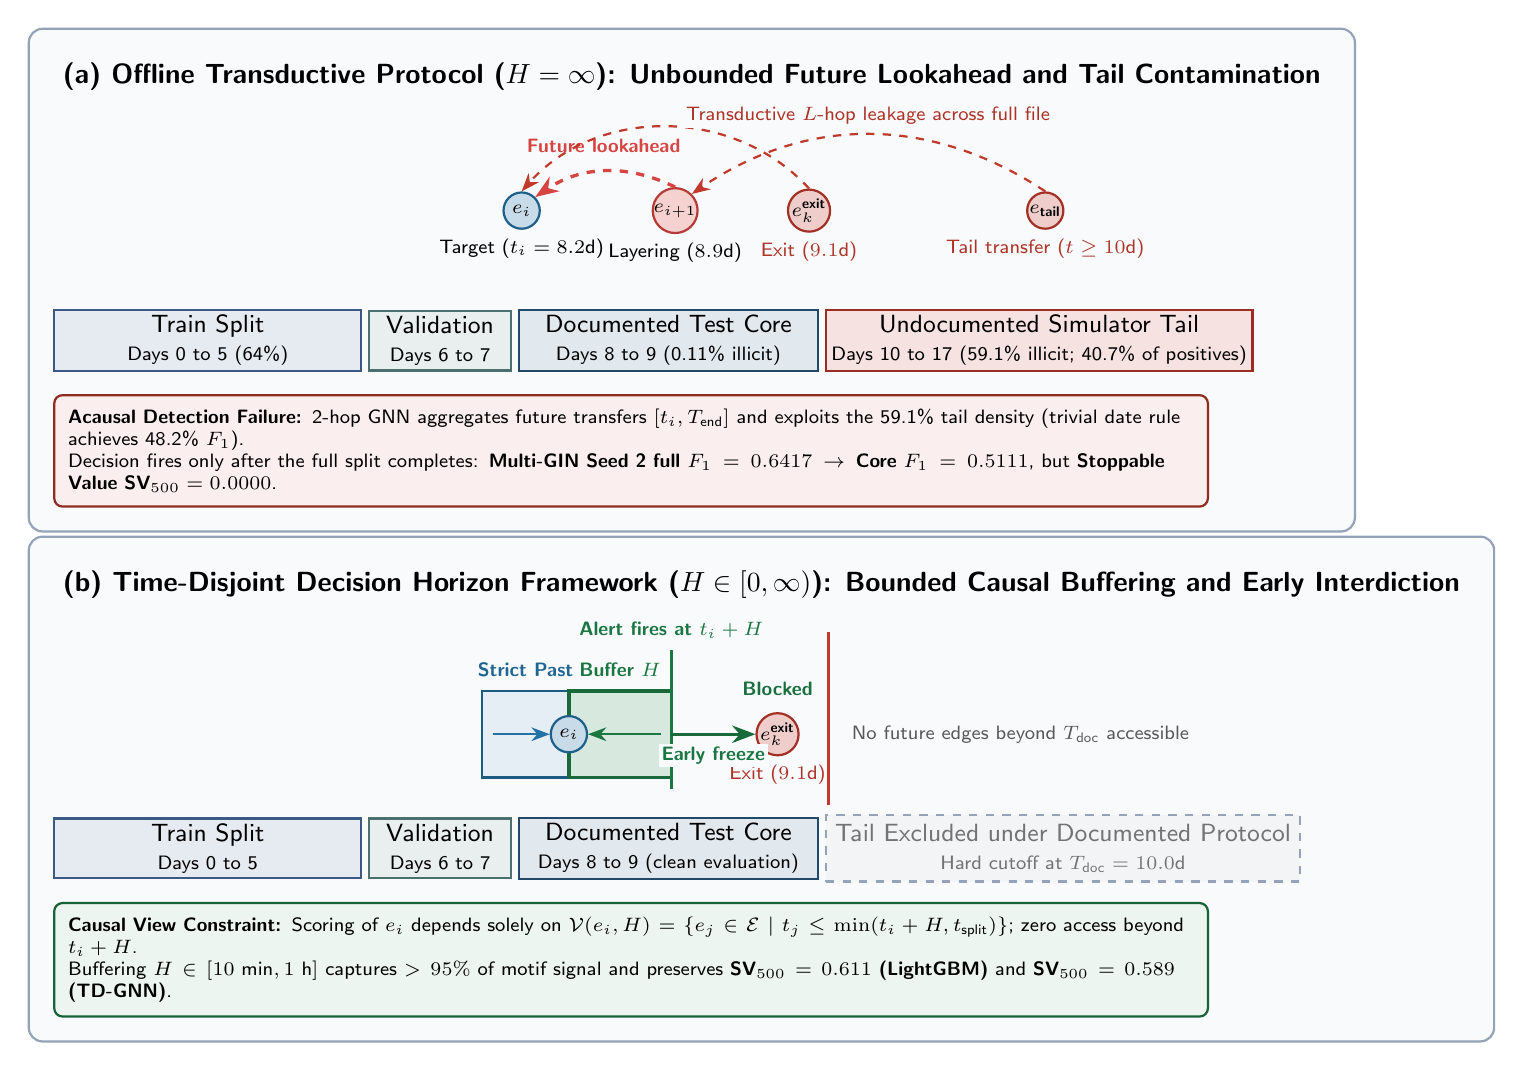
\begin{tikzpicture}[
    font=\sffamily\small,
    >=Stealth,
    zone/.style={rectangle, draw=#1!80!black, fill=#1!14, thick, minimum height=0.72cm, inner sep=2pt, align=center},
    ev/.style={circle, draw=#1!85!black, fill=#1!25, thick, minimum size=0.46cm, inner sep=0pt, font=\sffamily\scriptsize\bfseries},
    callout/.style={rectangle, rounded corners=3pt, draw=#1!75!black, fill=#1!8, thick, align=left, inner sep=5pt, font=\sffamily\scriptsize},
    panelbox/.style={rectangle, rounded corners=5pt, draw=slateborder, fill=panelbg, thick, inner sep=9pt}
]

% =====================================================================
% PANEL (a): Transductive Offline Graph and Tail Contamination (H = inf)
% =====================================================================
\begin{scope}[local bounding box=panelA]
    \node[anchor=west, font=\sffamily\normalsize\bfseries, text=black] (titleA) at (0, 4.75)
        {(a) Offline Transductive Protocol ($H = \infty$): Unbounded Future Lookahead and Tail Contamination};

    % Timeline bar (y = 1.40)
    \node[zone=traincol, minimum width=3.9cm, anchor=west] (trA) at (0, 1.40) {Train Split\\[-1pt]\scriptsize Days 0 to 5 (64\%)};
    \node[zone=valcol, minimum width=1.8cm, anchor=west] (vaA) at (4.0, 1.40) {Validation\\[-1pt]\scriptsize Days 6 to 7};
    \node[zone=corecol, minimum width=3.8cm, anchor=west] (coA) at (5.9, 1.40) {Documented Test Core\\[-1pt]\scriptsize Days 8 to 9 (0.11\% illicit)};
    \node[zone=tailcol, minimum width=4.9cm, anchor=west] (taA) at (9.8, 1.40) {Undocumented Simulator Tail\\[-1pt]\scriptsize Days 10 to 17 (59.1\% illicit; 40.7\% of positives)};

    % Event nodes in elevated band (y = 3.05) completely clear of timeline bar
    \node[ev=pastcol] (eiA) at (5.95, 3.05) {$e_i$};
    \node[below=2pt of eiA, font=\sffamily\scriptsize, fill=panelbg, inner sep=1pt] {Target ($t_i = 8.2\text{d}$)};

    \node[ev=leakcol] (efA) at (7.90, 3.05) {$e_{i+1}$};
    \node[below=2pt of efA, font=\sffamily\scriptsize, fill=panelbg, inner sep=1pt] {Layering ($8.9\text{d}$)};

    \node[ev=tailcol] (exA) at (9.60, 3.05) {$e_k^{\text{exit}}$};
    \node[below=2pt of exA, font=\sffamily\scriptsize, text=tailcol!90!black, fill=panelbg, inner sep=1pt] {Exit ($9.1\text{d}$)};

    \node[ev=tailcol] (etA) at (12.60, 3.05) {$e_{\text{tail}}$};
    \node[below=2pt of etA, font=\sffamily\scriptsize, text=tailcol!90!black, fill=panelbg, inner sep=1pt] {Tail transfer ($t \ge 10\text{d}$)};

    % Backward acausal message passing arcs routed cleanly ABOVE y = 3.05
    \draw[->, leakcol, very thick, dashed, bend right=30] (efA.north) to
        node[above, font=\sffamily\scriptsize\bfseries, text=leakcol, yshift=3pt] {Future lookahead} (eiA.north east);
    \draw[->, tailcol, thick, dashed, bend right=48] (exA.north) to (eiA.north);
    \draw[->, tailcol, thick, dashed, bend right=34] (etA.north) to
        node[above, font=\sffamily\scriptsize, text=tailcol!90!black, fill=panelbg, inner sep=1.5pt, yshift=2pt]
        {Transductive $L$-hop leakage across full file} (efA.north east);

    % Alert outcome callout (y = 0.65 down)
    \node[callout=tailcol, anchor=north west, text width=14.3cm] (outA) at (0, 0.72) {%
        \textbf{Acausal Detection Failure:} 2-hop GNN aggregates future transfers $[t_i, T_{\text{end}}]$ and exploits the 59.1\% tail density (trivial date rule achieves 48.2\% $F_1$).\\
        Decision fires only after the full split completes: \textbf{Multi-GIN Seed 2 full $F_1 = 0.6417 \to \text{Core } F_1 = 0.5111$}, but \textbf{Stoppable Value $\text{SV}_{500} = 0.0000$}.
    };
\end{scope}

% =====================================================================
% PANEL (b): Causal Time-Disjoint Decision Horizon (H >= 0)
% =====================================================================
\begin{scope}[yshift=-6.45cm, local bounding box=panelB]
    \node[anchor=west, font=\sffamily\normalsize\bfseries, text=black] (titleB) at (0, 4.75)
        {(b) Time-Disjoint Decision Horizon Framework ($H \in [0, \infty)$): Bounded Causal Buffering and Early Interdiction};

    % Timeline bar (y = 1.40)
    \node[zone=traincol, minimum width=3.9cm, anchor=west] (trB) at (0, 1.40) {Train Split\\[-1pt]\scriptsize Days 0 to 5};
    \node[zone=valcol, minimum width=1.8cm, anchor=west] (vaB) at (4.0, 1.40) {Validation\\[-1pt]\scriptsize Days 6 to 7};
    \node[zone=corecol, minimum width=3.8cm, anchor=west] (coB) at (5.9, 1.40) {Documented Test Core\\[-1pt]\scriptsize Days 8 to 9 (clean evaluation)};
    \node[rectangle, draw=slateborder, fill=slateborder!12, dashed, thick, minimum width=4.9cm, minimum height=0.72cm, anchor=west, align=center, text=black!55] (taB) at (9.8, 1.40) {Tail Excluded under Documented Protocol\\[-1pt]\scriptsize Hard cutoff at $T_{\text{doc}} = 10.0\text{d}$};

    % Receptive field shading in elevated band (y = 2.30 to 3.40)
    \fill[pastcol!12] (5.45, 2.30) rectangle (6.55, 3.40);
    \fill[safecol!18] (6.55, 2.30) rectangle (7.85, 3.40);
    \draw[pastcol!80!black, thick] (5.45, 2.30) rectangle (6.55, 3.40);
    \draw[safecol!80!black, very thick] (6.55, 2.30) rectangle (7.85, 3.40);

    \node[anchor=south, font=\sffamily\scriptsize\bfseries, text=pastcol!90!black] at (6.00, 3.46) {Strict Past};
    \node[anchor=south, font=\sffamily\scriptsize\bfseries, text=safecol!90!black] at (7.20, 3.46) {Buffer $H$};

    % Target event and vertical trigger wall
    \node[ev=pastcol] (eiB) at (6.55, 2.85) {$e_i$};
    \draw[very thick, safecol!90!black] (7.85, 2.15) -- (7.85, 3.92);
    \node[anchor=south, font=\sffamily\scriptsize\bfseries, text=safecol!90!black] at (7.85, 3.94) {Alert fires at $t_i + H$};

    % Causal information arrows inside the boxes
    \draw[->, pastcol, thick] (5.58, 2.85) -- (eiB.west);
    \draw[->, safecol!90!black, thick] (7.72, 2.85) -- (eiB.east);

    % Blocked exit event well separated before vertical wall at 9.80
    \node[ev=tailcol] (exB) at (9.20, 2.85) {$e_k^{\text{exit}}$};
    \node[below=2pt of exB, font=\sffamily\scriptsize, text=tailcol!90!black, fill=panelbg, inner sep=1pt] {Exit ($9.1\text{d}$)};
    \node[anchor=south, font=\sffamily\scriptsize\bfseries, text=safecol!85!black] at (9.20, 3.22) {Blocked};

    % Arrow from trigger wall to blocked exit, label cleanly below
    \draw[->, safecol!80!black, very thick] (7.85, 2.85) -- (exB.west)
        node[midway, below=3pt, font=\sffamily\scriptsize\bfseries, text=safecol!90!black, fill=panelbg, inner sep=1pt] {Early freeze};

    % Hard documented boundary wall separating core from tail
    \draw[tailcol, very thick] (9.85, 1.95) -- (9.85, 4.15);
    \node[anchor=west, font=\sffamily\scriptsize, text=black!65] at (10.02, 2.85) {No future edges beyond $T_{\text{doc}}$ accessible};

    % Horizon outcome callout
    \node[callout=safecol, anchor=north west, text width=14.3cm] (outB) at (0, 0.72) {%
        \textbf{Causal View Constraint:} Scoring of $e_i$ depends solely on $\mathcal{V}(e_i, H) = \{e_j \in \mathcal{E} \mid t_j \le \min(t_i + H, t_{\text{split}})\}$; zero access beyond $t_i + H$.\\
        Buffering $H \in [10\text{ min}, 1\text{ h}]$ captures $>95\%$ of motif signal and preserves \textbf{$\text{SV}_{500} = 0.611$ (LightGBM)} and \textbf{$\text{SV}_{500} = 0.589$ (TD-GNN)}.
    };
\end{scope}

% Background frame around both panels
\begin{scope}[on background layer]
    \node[panelbox, fit=(panelA)] {};
    \node[panelbox, fit=(panelB)] {};
\end{scope}

\end{tikzpicture}
\end{document}
